\documentclass[aspectratio=169]{beamer}
\usetheme{Madrid}
\usecolortheme{default}

% Packages
\usepackage{graphicx}
\usepackage{booktabs}
\usepackage{amsmath}
\usepackage{hyperref}
\usepackage{tikz}
\usepackage{pgfplots}
\pgfplotsset{compat=1.18}

% Title page information
\title[EITC and Labor Supply]{Labor Supply Response to the Earned Income Tax Credit}
\subtitle{Eissa \& Liebman (1996) \\ \textit{Quarterly Journal of Economics}}
\author{Juan Cosme}
\institute{University of South Florida}
\date{\ November 12, 2025}

\begin{document}

% Title slide
\begin{frame}
\titlepage
\end{frame}

% Slide 1: Primary Research Question
\begin{frame}{Primary Research Question}
\vspace{1cm}
\begin{center}
\LARGE
\textbf{Does the Earned Income Tax Credit (EITC) \\increase labor force participation \\among single mothers?}
\end{center}

\vspace{1cm}
\begin{itemize}
    \item Focus: Extensive margin (whether to work)
    \item Policy change: 1986 Tax Reform Act (TRA86)
    \item Population: Single women with children
\end{itemize}
\end{frame}

% Slide 2: Background and Motivation
\begin{frame}{Background and Motivation}
\textbf{What is the EITC?}
\begin{itemize}
    \item Refundable tax credit for low-to-moderate income working families
    \item Largest anti-poverty program in the United States
    \item Designed to "make work pay" by supplementing earnings
    \item Must have earned income to qualify
\end{itemize}

\vspace{0.5cm}
\textbf{Why does this matter?}
\begin{itemize}
    \item Understanding work incentives vs. income support
    \item Policy design: Does the EITC achieve its goals?
    \item Budget implications: Self-financing through increased employment?
    \item Alternative to traditional welfare programs
\end{itemize}
\end{frame}

% Slide 3: Research Design
\begin{frame}{Research Design}
\textbf{Natural Experiment Approach:}
\begin{itemize}
    \item \textbf{Treatment group:} Single mothers (eligible for EITC)
    \item \textbf{Control group:} Single women without children (not eligible)
    \item \textbf{Policy shock:} TRA86 expanded EITC by 60\% in real terms
    \item \textbf{Method:} Difference-in-Differences (DD)
\end{itemize}

\vspace{0.5cm}
\begin{center}
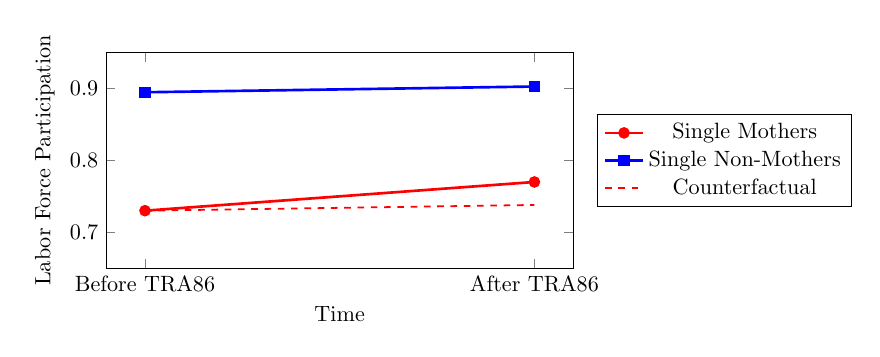
\begin{tikzpicture}[scale=0.8]
\begin{axis}[
    xlabel={Time},
    ylabel={Labor Force Participation},
    symbolic x coords={Before TRA86, After TRA86},
    xtick=data,
    ymin=0.65, ymax=0.95,
    legend style={at={(1.05,0.5)}, anchor=west},
    width=9cm,
    height=5cm
]
\addplot[color=red, very thick, mark=*] coordinates {
    (Before TRA86, 0.73)
    (After TRA86, 0.77)
};
\addplot[color=blue, very thick, mark=square*] coordinates {
    (Before TRA86, 0.895)
    (After TRA86, 0.903)
};
\addplot[color=red, dashed, thick] coordinates {
    (Before TRA86, 0.73)
    (After TRA86, 0.738)
};
\legend{Single Mothers, Single Non-Mothers, Counterfactual}
\end{axis}
\end{tikzpicture}
\end{center}
\end{frame}

% Slide 4: Identification Strategy
\begin{frame}{Identification Strategy}
\textbf{Key Identifying Assumption: Parallel Trends}
\begin{itemize}
    \item Without TRA86, both groups would have followed similar trends
    \item Single mothers and non-mothers are similar demographically
    \item Both groups face similar macroeconomic conditions
    \item EITC eligibility based solely on having children
\end{itemize}

\vspace{0.5cm}
\textbf{What creates exogenous variation?}
\begin{itemize}
    \item TRA86 was a federal policy change (exogenous to individuals)
    \item Large, discrete increase in benefits (60\% real increase)
    \item Maximum credit: \$550 (1986) → \$953 (1990)
    \item Clear eligibility rules based on children
\end{itemize}
\end{frame}

% Slide 5: Regression Specification
\begin{frame}{Regression Specification}
\textbf{Difference-in-Differences Model:}

\vspace{0.3cm}
\begin{equation*}
P(LFP_{it} = 1) = \Phi(\beta_0 + \beta_1 \cdot ANYKIDS_i + \beta_2 \cdot POST86_t + \beta_3 \cdot (ANYKIDS_i \times POST86_t) + X_{it}'\gamma)
\end{equation*}

\vspace{0.5cm}
\textbf{Where:}
\begin{itemize}
    \item $\Phi$ = Standard normal CDF (Probit model)
    \item $ANYKIDS_i$ = 1 if woman has children, 0 otherwise
    \item $POST86_t$ = 1 if year is 1988-1990, 0 if 1984-1986
    \item $\beta_3$ = \textbf{DD estimate} (our coefficient of interest)
    \item $X_{it}$ = Controls (age, education, race, state unemployment, AFDC)
\end{itemize}

\vspace{0.3cm}
\textbf{Interpretation:} $\beta_3$ captures the differential change in labor force participation for single mothers relative to single non-mothers after TRA86
\end{frame}

% Slide 6: Testing Parallel Trends
\begin{frame}{Testing Parallel Trends}
\textbf{Pre-Treatment Trends (1979-1986):}
\begin{itemize}
    \item Both groups show similar trends before TRA86
    \item No differential trends in pre-reform period
    \item Validates parallel trends assumption
    \item Effects emerge only after 1986
\end{itemize}

\vspace{0.3cm}
\begin{center}
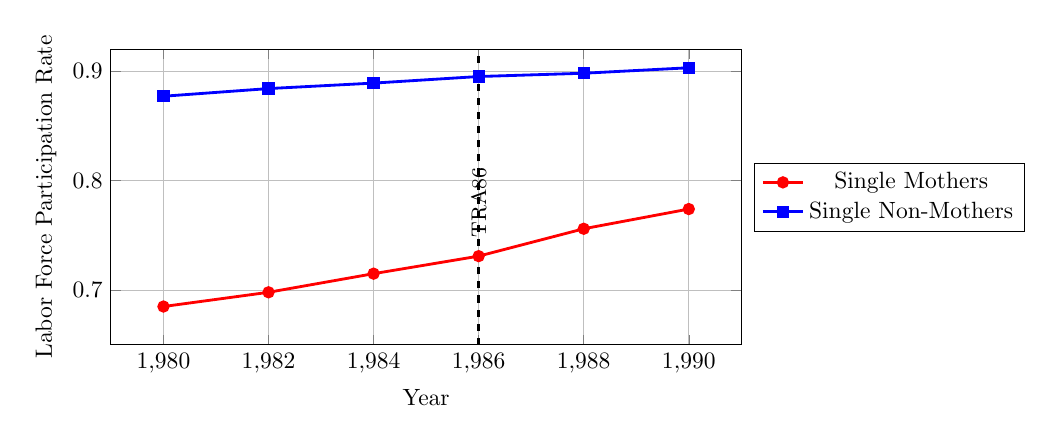
\begin{tikzpicture}[scale=0.85]
\begin{axis}[
    xlabel={Year},
    ylabel={Labor Force Participation Rate},
    xmin=1979, xmax=1991,
    ymin=0.65, ymax=0.92,
    xtick={1980,1982,1984,1986,1988,1990},
    legend style={at={(1.02,0.5)}, anchor=west},
    grid=major,
    width=11cm,
    height=6cm
]
\addplot[color=red, very thick, mark=*] coordinates {
    (1980,0.685) (1982,0.698) (1984,0.715) (1986,0.731)
    (1988,0.756) (1990,0.774)
};
\addplot[color=blue, very thick, mark=square*] coordinates {
    (1980,0.877) (1982,0.884) (1984,0.889) (1986,0.895)
    (1988,0.898) (1990,0.903)
};
\addplot[black, dashed, very thick] coordinates {(1986,0.65) (1986,0.92)};
\node[anchor=south, rotate=90] at (axis cs:1986.3,0.78) {\small TRA86};
\legend{Single Mothers, Single Non-Mothers}
\end{axis}
\end{tikzpicture}
\end{center}
\end{frame}

% Slide 7: Data
\begin{frame}{Data}
\textbf{Data Source:}
\begin{itemize}
    \item Current Population Survey (CPS) March Annual Demographic Files
    \item Years: 1984-1986 (pre-reform) and 1988-1990 (post-reform)
    \item 1987 excluded as transition year
\end{itemize}

\vspace{0.3cm}
\textbf{Sample:}
\begin{itemize}
    \item Single women aged 19-44
    \item Treatment: Single mothers ($n \approx$ 28,000)
    \item Control: Single non-mothers ($n \approx$ 24,000)
    \item Excluded: Students, disabled, armed forces
\end{itemize}

\vspace{0.3cm}
\textbf{Key Variables:}
\begin{itemize}
    \item Labor force participation (primary outcome)
    \item Hours worked, weeks worked
    \item Demographics: age, education, race, number of children
    \item State-level: unemployment rate, AFDC maximum benefits
\end{itemize}
\end{frame}

% Slide 8: Summary Statistics
\begin{frame}{Summary Statistics}
\begin{table}
\centering
\small
\begin{tabular}{lcccc}
\toprule
& \multicolumn{2}{c}{\textbf{Single Mothers}} & \multicolumn{2}{c}{\textbf{Single Non-Mothers}} \\
\cmidrule(lr){2-3} \cmidrule(lr){4-5}
\textbf{Variable} & \textbf{Pre-TRA86} & \textbf{Post-TRA86} & \textbf{Pre-TRA86} & \textbf{Post-TRA86} \\
\midrule
Labor force participation & 0.731 & 0.758 & 0.895 & 0.903 \\
Age & 32.1 & 32.8 & 28.5 & 29.3 \\
Less than high school & 0.234 & 0.203 & 0.149 & 0.123 \\
High school & 0.434 & 0.413 & 0.391 & 0.367 \\
Some college & 0.218 & 0.241 & 0.276 & 0.298 \\
College graduate & 0.114 & 0.143 & 0.184 & 0.212 \\
Nonwhite & 0.385 & 0.392 & 0.228 & 0.241 \\
Number of children & 1.89 & 1.83 & — & — \\
\midrule
Sample size & 13,747 & 14,333 & 11,568 & 12,742 \\
\bottomrule
\end{tabular}
\end{table}

\vspace{0.3cm}
\small
\textbf{Key observations:} Single mothers increased LFP by 2.7 pp; single non-mothers by 0.8 pp. \\
Difference-in-differences = 2.7 - 0.8 = \textbf{1.9 pp} (unconditional estimate)
\end{frame}

% Slide 9: Main Regression Results
\begin{frame}{Main Regression Results: Labor Force Participation}
\begin{table}
\centering
\begin{tabular}{lcc}
\toprule
\textbf{Specification} & \textbf{DD Estimate} & \textbf{Std. Error} \\
\midrule
\multicolumn{3}{l}{\textit{Panel A: Linear Probability Model}} \\
\quad Basic (no controls) & 0.029*** & (0.006) \\
\quad Add demographics & 0.028*** & (0.006) \\
\quad Add state controls & 0.027*** & (0.006) \\
\quad Full specification & 0.028*** & (0.006) \\
\addlinespace
\multicolumn{3}{l}{\textit{Panel B: Probit Model (Marginal Effects)}} \\
\quad Basic (no controls) & 0.030*** & (0.006) \\
\quad Full specification & 0.027*** & (0.006) \\
\bottomrule
\end{tabular}
\end{table}

\vspace{0.5cm}
\textbf{Main Finding:} EITC expansion increased labor force participation by \textbf{2.8 percentage points}

\vspace{0.2cm}
\small
Note: *** p$<$0.01. Estimates are remarkably stable across specifications.
\end{frame}

% Slide 10: Heterogeneous Treatment Effects
\begin{frame}{Heterogeneous Treatment Effects by Education}
\begin{columns}
\begin{column}{0.48\textwidth}
\begin{table}
\centering
\small
\begin{tabular}{lc}
\toprule
\textbf{Education Level} & \textbf{Effect (pp)} \\
\midrule
Less than HS & 6.7*** \\
 & (1.2) \\
\addlinespace
High school & 3.5*** \\
 & (0.9) \\
\addlinespace
Some college & 1.4 \\
 & (1.1) \\
\addlinespace
College grad & -0.1 \\
 & (1.3) \\
\bottomrule
\end{tabular}
\end{table}
\end{column}

\begin{column}{0.48\textwidth}
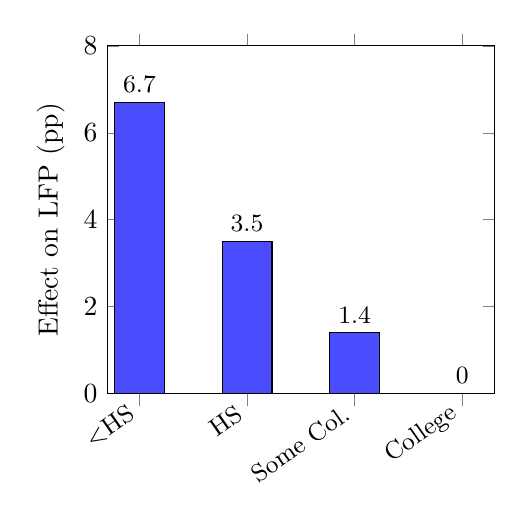
\begin{tikzpicture}
\begin{axis}[
    ybar,
    ylabel={Effect on LFP (pp)},
    symbolic x coords={$<$HS, HS, Some Col., College},
    xtick=data,
    x tick label style={font=\small, rotate=35, anchor=east},
    ymin=0, ymax=8,
    width=6.5cm,
    height=6cm,
    bar width=18pt,
    nodes near coords,
    every node near coord/.append style={font=\small}
]
\addplot[fill=blue!70] coordinates {
    ($<$HS, 6.7)
    (HS, 3.5)
    (Some Col., 1.4)
    (College, 0)
};
\end{axis}
\end{tikzpicture}
\end{column}
\end{columns}

\vspace{0.3cm}
\small
\textbf{Interpretation:} Largest effects for low-education women most likely to be EITC-eligible. Evidence of effective targeting.
\end{frame}

% Slide 11: Intensive vs Extensive Margin
\begin{frame}{Effects on Intensive vs. Extensive Margin}
\begin{columns}
\begin{column}{0.5\textwidth}
\textbf{Extensive Margin (Participation):}
\begin{itemize}
    \item \textcolor{green!70!black}{\textbf{Strong positive effect}}
    \item 2.8 pp increase in LFP
    \item Statistically significant
    \item $\sim$500,000 additional workers
\end{itemize}

\vspace{0.5cm}
\textbf{Intensive Margin (Hours Worked):}
\begin{itemize}
    \item \textcolor{red!70!black}{\textbf{No significant effect}}
    \item Minimal change in hours
    \item Among those already working
\end{itemize}
\end{column}

\begin{column}{0.5\textwidth}
\begin{table}
\centering
\small
\begin{tabular}{lcc}
\toprule
\textbf{Outcome} & \textbf{Coef.} & \textbf{SE} \\
\midrule
\multicolumn{3}{l}{\textit{Extensive Margin:}} \\
LFP & 0.028*** & (0.006) \\
\addlinespace
\multicolumn{3}{l}{\textit{Intensive Margin:}} \\
Annual hours (all) & 44.5 & (28.3) \\
Weekly hours (workers) & -0.15 & (0.31) \\
\bottomrule
\end{tabular}
\end{table}

\vspace{0.3cm}
\begin{block}{Why?}
\small
Income and substitution effects offset on intensive margin
\end{block}
\end{column}
\end{columns}
\end{frame}

% Slide 12: Placebo Tests
\begin{frame}{Placebo Tests: Pre-TRA86 Periods}
\textbf{Testing for Spurious Differential Trends:}
\begin{itemize}
    \item Run "fake" DD regressions in periods before TRA86
    \item If parallel trends hold, should find no effects
    \item Validates that effects are truly due to EITC expansion
\end{itemize}

\vspace{0.3cm}
\begin{table}
\centering
\begin{tabular}{lccc}
\toprule
\textbf{Time Period Comparison} & \textbf{DD Estimate} & \textbf{Std. Error} & \textbf{Significant?} \\
\midrule
1982 vs. 1980 (Placebo) & 0.003 & (0.008) & No \\
1984 vs. 1982 (Placebo) & -0.001 & (0.008) & No \\
\addlinespace[0.2cm]
\textbf{1988-90 vs. 1984-86 (Actual)} & \textbf{0.028} & \textbf{(0.006)} & \textbf{Yes***} \\
\bottomrule
\end{tabular}
\end{table}

\vspace{0.3cm}
\textbf{Interpretation:}
\begin{itemize}
    \item No differential trends before TRA86
    \item Significant effect only after policy change
    \item Strengthens causal interpretation
\end{itemize}
\end{frame}

% Slide 13: Robustness Checks
\begin{frame}{Robustness Checks}
\textbf{Alternative Specifications:}
\begin{itemize}
    \item Probit vs. linear probability model → Consistent results
    \item Different sets of control variables → Stable estimates
    \item Alternative time windows → Similar findings
    \item State-specific trends → Results hold
\end{itemize}

\vspace{0.3cm}
\textbf{Alternative Control Groups:}
\begin{itemize}
    \item Primary: Single women without children
    \item Alternative: Married women with children (less ideal)
    \item Results robust across control groups
\end{itemize}

\vspace{0.3cm}
\textbf{Sample Restrictions:}
\begin{itemize}
    \item Different age ranges (25-44, 19-54)
    \item Exclude specific demographic groups
    \item Results qualitatively unchanged
\end{itemize}
\end{frame}

% Slide 14: Policy Implications
\begin{frame}{Policy Implications}
\textbf{For EITC Policy:}
\begin{itemize}
    \item EITC successfully achieves its goal of increasing employment
    \item Work-based assistance more effective than traditional welfare
    \item Evidence supports further EITC expansions (1990, 1993, 2001, 2009)
\end{itemize}

\vspace{0.3cm}
\textbf{Budget Implications:}
\begin{itemize}
    \item Program partially self-financing through increased employment
    \item Additional workers generate tax revenue
    \item Cost per new worker: \$3,000-\$5,000
    \item More cost-effective than traditional welfare
\end{itemize}

\vspace{0.3cm}
\textbf{Broader Impact:}
\begin{itemize}
    \item Informed 1996 welfare reform (PRWORA)
    \item Model for other countries (UK, Canada, France)
    \item Demonstrates work incentives can be effective
\end{itemize}
\end{frame}

% Slide 15: Limitations
\begin{frame}{Limitations and Challenges}
\textbf{Study Limitations:}
\begin{enumerate}
    \item \textbf{Short-run effects only:} Cannot speak to long-term career trajectories
    \item \textbf{Single mothers only:} Doesn't examine effects on other family types
    \item \textbf{Extensive margin focus:} Limited analysis of job quality and wages
    \item \textbf{General equilibrium:} Ignores wage effects and worker displacement
    \item \textbf{Mechanisms unclear:} How did women learn about EITC changes?
\end{enumerate}

\vspace{0.3cm}
\textbf{Threats to Identification:}
\begin{itemize}
    \item Other policies affecting single mothers (AFDC changes)
    \item Compositional changes in who becomes a single mother
    \item Potential spillovers to control group
\end{itemize}
\end{frame}

% Slide 16: Future Research Directions
\begin{frame}{Suggestions for Future Research}
\textbf{Extensions Identified by Authors:}
\begin{enumerate}
    \item Long-term effects on earnings and career progression
    \item Children's outcomes (education, health, development)
    \item Effects on marriage decisions and family structure
    \item Job quality, wages, and occupation choice
    \item General equilibrium effects on wages
\end{enumerate}

\vspace{0.3cm}
\textbf{Subsequent Literature Addressed:}
\begin{itemize}
    \item Meyer \& Rosenbaum (2001): 1990s EITC expansions
    \item Eissa \& Hoynes (2004): Effects on married couples
    \item Chetty et al. (2013): Tax filing and information
    \item Bastian \& Michelmore (2018): Long-term child outcomes
    \item Rothstein (2010): Wage incidence
\end{itemize}
\end{frame}

% Slide 17: Conclusion
\begin{frame}{Conclusion}
\textbf{Main Contributions:}
\begin{enumerate}
    \item \textbf{First credible causal evidence} that EITC increases employment
    \item \textbf{Methodological innovation:} Natural experiment approach using tax reform
    \item \textbf{Policy impact:} Informed subsequent EITC expansions and welfare reform
    \item \textbf{Framework:} Established DD methodology for tax policy evaluation
\end{enumerate}

\vspace{0.5cm}
\begin{block}{Bottom Line}
The EITC expansion increased labor force participation of single mothers by 2.8 percentage points, bringing approximately 500,000 additional women into the workforce. The program achieves its dual goals of poverty reduction and employment promotion.
\end{block}

\vspace{0.3cm}
\textbf{Key Insight:} Well-designed wage subsidies can enhance both equity and efficiency
\end{frame}

% Slide 18: Appendix - EITC Schedule
\begin{frame}{Appendix: EITC Benefit Schedule}
\begin{center}
\textbf{Figure A1: EITC Credit Amount by Earnings Level}
\vspace{0.3cm}

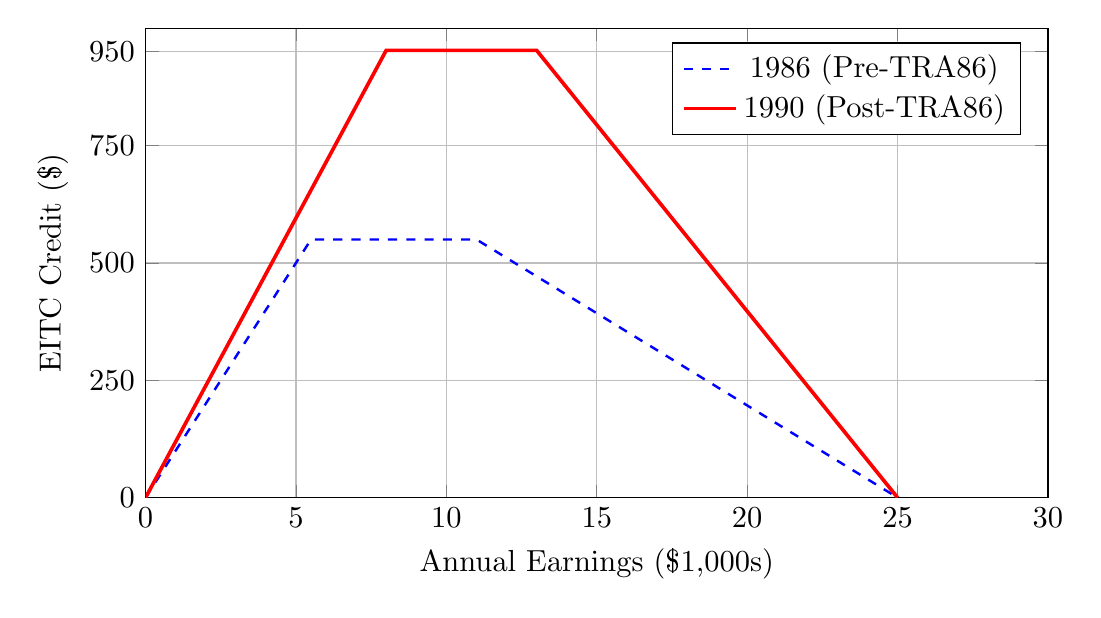
\begin{tikzpicture}[scale=1.1]
\begin{axis}[
    xlabel={Annual Earnings (\$1,000s)},
    ylabel={EITC Credit (\$)},
    xmin=0, xmax=30,
    ymin=0, ymax=1000,
    xtick={0,5,10,15,20,25,30},
    ytick={0,250,500,750,950},
    legend pos=north east,
    grid=major,
    width=12cm,
    height=7cm
]
% 1986 schedule
\addplot[color=blue, thick, dashed] coordinates {
    (0,0) (5.5,550) (11,550) (25,0)
};
% 1990 schedule  
\addplot[color=red, very thick] coordinates {
    (0,0) (8,953) (13,953) (25,0)
};
\legend{1986 (Pre-TRA86), 1990 (Post-TRA86)}
\end{axis}
\end{tikzpicture}

\vspace{0.3cm}
\small
Note: TRA86 increased maximum credit from \$550 to \$953 (73\% nominal increase, 60\% real increase)
\end{center}
\end{frame}

% Slide 19: Appendix - Full Regression Table
\begin{frame}{Appendix: Full Regression Results}
\begin{table}
\centering
\scriptsize
\begin{tabular}{lcccc}
\toprule
& \textbf{(1)} & \textbf{(2)} & \textbf{(3)} & \textbf{(4)} \\
& \textbf{Basic} & \textbf{+ Demo} & \textbf{+ State} & \textbf{Full} \\
\midrule
ANYKIDS $\times$ POST86 & 0.029*** & 0.028*** & 0.027*** & 0.028*** \\
 & (0.006) & (0.006) & (0.006) & (0.006) \\
\addlinespace
ANYKIDS & -0.164*** & -0.087*** & -0.086*** & -0.084*** \\
 & (0.004) & (0.005) & (0.005) & (0.005) \\
\addlinespace
POST86 & 0.008** & 0.012*** & 0.011*** & 0.010** \\
 & (0.004) & (0.004) & (0.004) & (0.004) \\
\addlinespace
Age & & 0.025*** & 0.025*** & 0.024*** \\
 & & (0.002) & (0.002) & (0.002) \\
\addlinespace
Education controls & No & Yes & Yes & Yes \\
Race controls & No & Yes & Yes & Yes \\
State unemployment & No & No & Yes & Yes \\
AFDC benefits & No & No & Yes & Yes \\
Year fixed effects & Yes & Yes & Yes & Yes \\
State fixed effects & No & No & No & Yes \\
\addlinespace
Observations & 52,390 & 52,390 & 52,390 & 52,390 \\
R-squared & 0.082 & 0.145 & 0.147 & 0.163 \\
\bottomrule
\end{tabular}
\end{table}

\vspace{0.2cm}
\tiny
Note: Robust standard errors in parentheses. *** p$<$0.01, ** p$<$0.05, * p$<$0.1
\end{frame}

% Slide 20: Questions
\begin{frame}[standout]
\begin{center}
\Huge Questions?
\end{center}
\end{frame}

\end{document}